\subsection{Resumo}

\begin{table}[h!]
\centering
\begin{tabular}{ |c|c|c|c|c|  }
\hline
\rowcolor{lightgray}
Algoritmo & Max & Min & Média & Desvio Padrão \\
\hline
Hill-Climbing & 37.674 & -8.424 & 7.498 & 13.852 \\
\hline
Hill-Climbing com restart & -6.452 & -9.997 & -9.297 & 1.131 \\
\hline
Simulated Annealing & 15.216 & -10.0 & -2.956 & 8.794 \\
\hline
Genetic Algorithm & -9.821 & -10.0 & -9.96 & 0.068 \\
\hline

\end{tabular}
\caption{Tabela com dados consolidados dos algoritmos}
\end{table}

\begin{figure}[H]
\centering
  \begin{minipage}[b]{0.48\textwidth}
    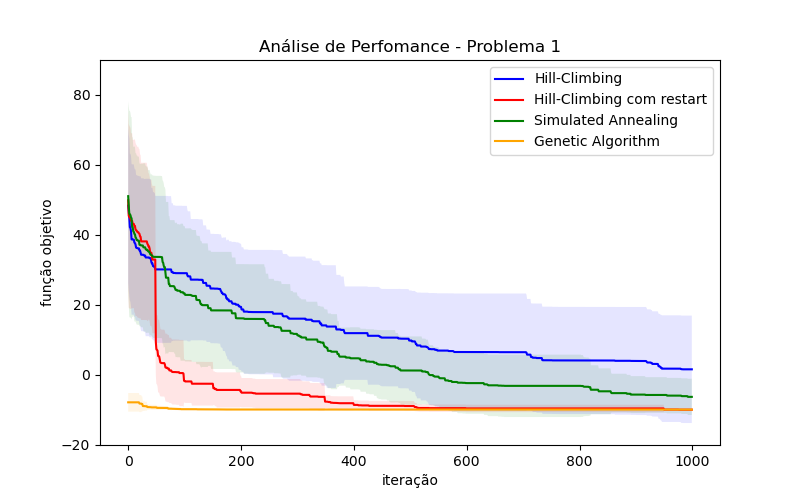
\includegraphics[width=88mm]{imagens/otima/problema-1-performance-algoritmos-best.png}
    \caption{Dados da execução da função objetivo durante as 10 iterações por melhor valor.
    \label{fig:problema-1-performance-algoritmos-best}}
  \end{minipage}
  \hfill
  \begin{minipage}[b]{0.48\textwidth}
    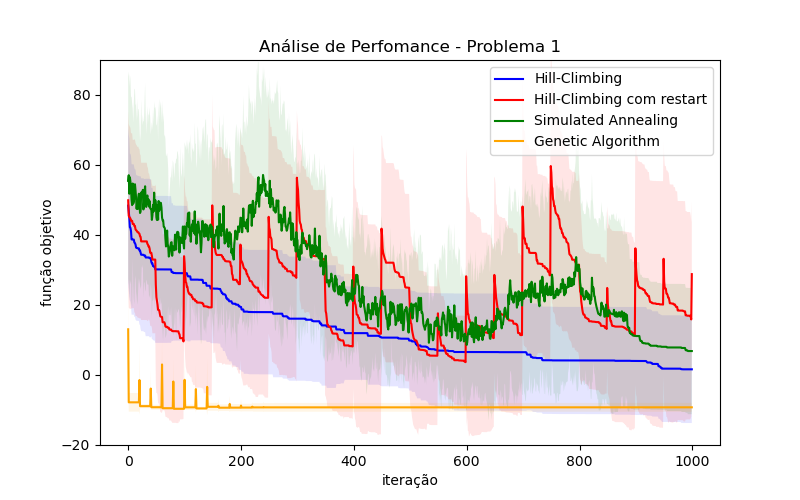
\includegraphics[width=88mm]{imagens/otima/problema-1-performance-algoritmos-value.png}
    \caption{Dados da execução da função objetivo durante as 10 iterações por valor atual.
    \label{fig:problema-1-performance-algoritmos-value}}
  \end{minipage}
\end{figure}